\section{Multiplexage}

\begin{frame}[fragile]
  \frametitle{Multiplexage}
\begin{center}
	\Huge{\bf\color{blue}Multiplexage}
\end{center}
\begin{flushright}
	\item Multiplexage fréquentiel
	\item Multiplexage par répartition orthogonale de la la fréquence
	\item Multiplexage temporel
	\item Multiplexage par répartition de codes
	\item Multiplexage en longueur d'ondes
\end{flushright}
\end{frame}


\begin{frame}[fragile]
  \frametitle{Multiplexage}
{\bf\large  Multiplexage}\\
Consiste à partager une même ligne entre plusieurs signaux
\par Il est inenvisageable de «tirer» une ligne par signal
\end{frame}


\section{Multiplexage fréquentiel (FDM)}

\begin{frame}[fragile]
  \frametitle{Multiplexage fréquentiel (FDM)}
{\bf\large Multiplexage fréquentiel 
(\textit{FDM Frequency Division Multiplexing})}\\
Division du spectre en bandes de fréquences
\begin{itemize}
	\item Basé sur la transmission «passe bande»
	\begin{itemize}
		\item Un signal qui occupe de 0 à B Hz peut être décalé pour occuper une
		fréquence de S à S+B Hz
	\end{itemize}
	\item Division du spectre en bandes de fréquences, chaque utilisateur a la
	possession exclusive d'une bande
\end{itemize}
\vspace{1cm}
Exemples
\begin{itemize}
	\item la radiodiffusion AM
	\item réseaux téléphoniques, cellulaires, sans fil et satellitaires
\end{itemize}
\end{frame}

\begin{frame}[fragile]
  \frametitle{Multiplexage fréquentiel (FDM)}
\begin{center}
	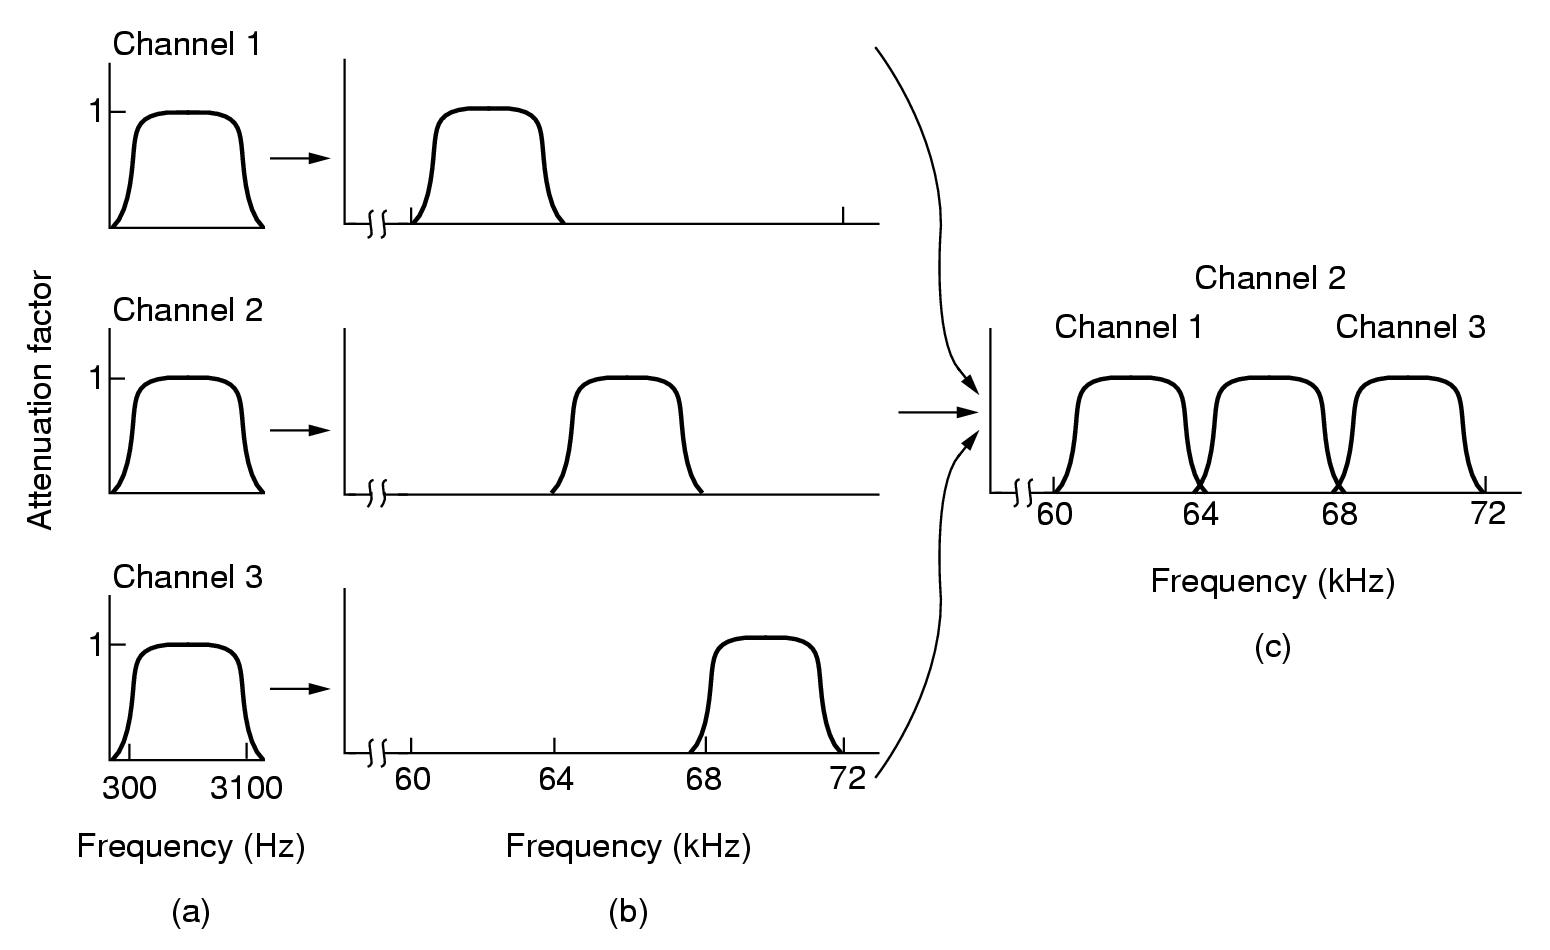
\includegraphics[width=.7\linewidth]{img/2-24.jpg}\\
	{\scriptsize FDM - Image de [Tanenbaum]}
\end{center}
\end{frame}

\begin{frame}[fragile]
	\frametitle{Transmission passe-bande}
{\large\bf Transmission passe-bande}
\par
En transmission passe-bande, la \textbf{modulation numérique} se fait en modifiant
\begin{itemize}
	\item l'amplitude (\textit{AFK Amplitude Shift Keying})
	\item la fréquence (\textit{FSK Frequence Shift Keying}) ou
	\item la phase (\textit{PSK Phase Shift Keying})
\end{itemize}
\end{frame}

\begin{frame}[fragile]
	\frametitle{Transmission passe-bande}
{\large\bf Transmission passe-bande}
\begin{center}
	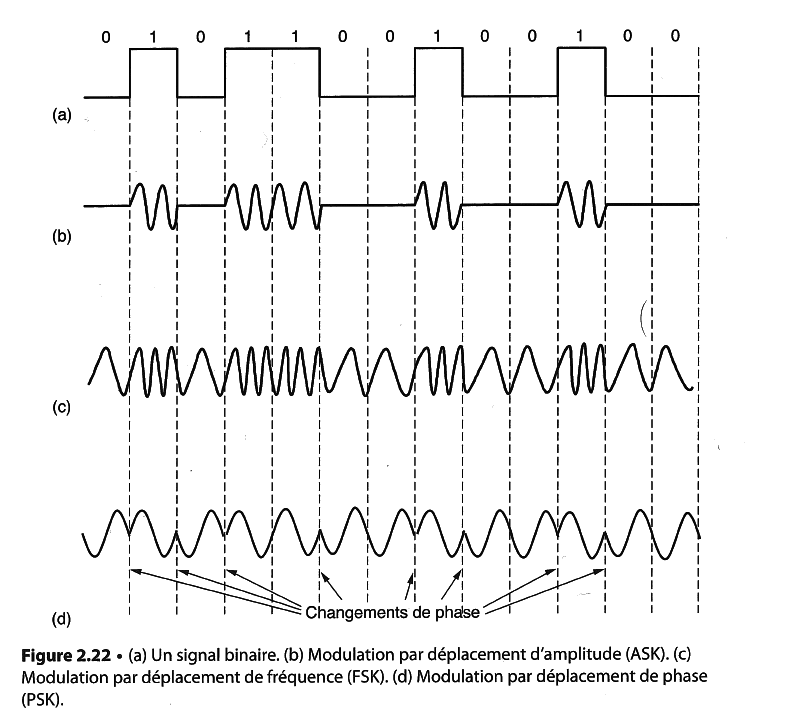
\includegraphics[width=.64\linewidth]{img/2-22.png} \\
	{\scriptsize From [Tanenbaum]}
\end{center}
\end{frame}

\begin{frame}[fragile]
	\frametitle{Transmission passe-bande}
{\large\bf \textit{BPSK Binary Phase Shift Keying}}
\begin{itemize}
	\item La porteuse est décalée de 0 ou $\pi$, soit \textbf{deux symboles}
	($\frac{2\pi}{2}$)
\end{itemize}
\vspace{1cm}
{\large\bf \textit{QPSK Quadrature Phase Shift Keying}}
\begin{itemize}
	\item On ne découpe plus en 2 mais en 4, soit 
	$\frac{\pi}{4}$, $\frac{3\pi}{4}$, $\frac{5\pi}{4}$ et $\frac{7\pi}{4}$
	\item Permet de représenter 4 symboles, soit 2 bits par symbole
\end{itemize}
\end{frame}

\begin{frame}[fragile]
	\frametitle{Transmission passe-bande}
{\large\bf \textit{QAM Quadrature Amplitude Modulation}}
\begin{itemize}
	\item Combinaison de PSK et AFK
	\item Permet de plusieurs symboles, on parle de \textbf{constellations}
\end{itemize}
\begin{center}
	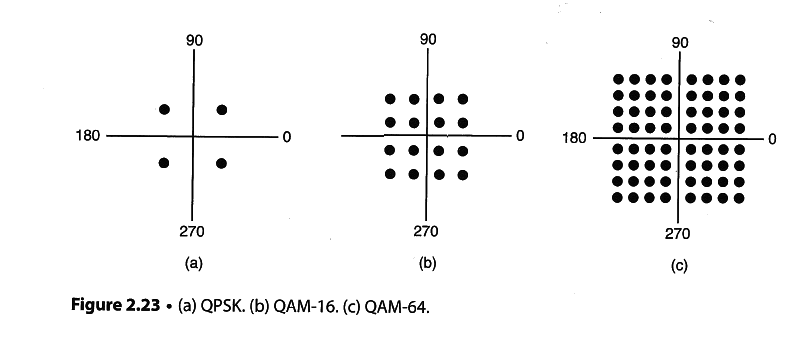
\includegraphics[width=.6\linewidth]{img/2-23.png}
\end{center}
\end{frame}

\begin{frame}[fragile]
	\frametitle{Transmission passe-bande}
{\large\bf \textit{QAM Quadrature Amplitude Modulation (suite)}}
\begin{itemize}
	\item QAM16, QAM64, ...
	\item Association des bits aux symboles de manière à minimiser 
	les erreurs dues au bruit, \textbf{code de Gray}
\end{itemize}
\begin{center}
	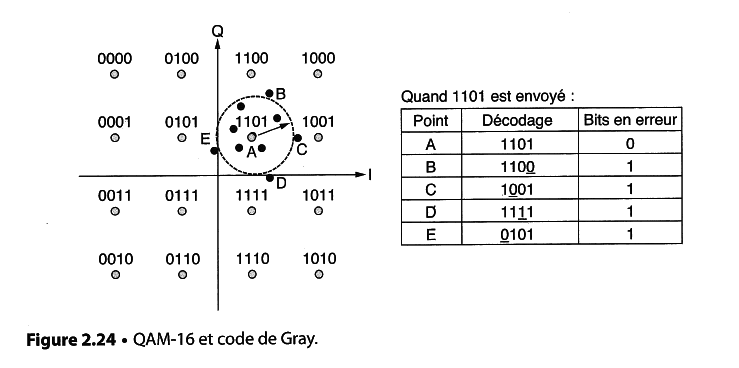
\includegraphics[width=.8\linewidth]{img/2-24.png}
\end{center}
\end{frame}

\section{Multiplexage par répartition orthogonal de la fréquence (OFDM)}

\begin{frame}[fragile]
  \frametitle{Multiplexage par répartition orthogonale de la fréquence (OFDM)}
{\large\bf Multiplexage par répartition orthogonale de la fréquence \\
(\textit{OFDM Orthogonal Frequency Division Multiplexing})}\\
Division du spectre en plusieurs sous-porteuses
\begin{itemize}
	\item Basé sur QAM (\textit{Quadrature Amplitude Modulation}), technique de
	modulation par variation de phase et de fréquence
	\item Les signaux de chaque sous porteuse se chevauchent mais s'annulent au
	centre car leurs fréquences sont orthogonales
\end{itemize}
\vspace{.6cm}
Exemples 
\begin{itemize}
	\item Très haut débit
	\item CPL (Courant porteur)
	\item 4G
	\item ADSL, VDSL
	\item câble
\end{itemize}
\end{frame}

\begin{frame}[fragile]
  \frametitle{Multiplexage par répartition orthogonale de la fréquence (OFDM)}
\begin{center}
	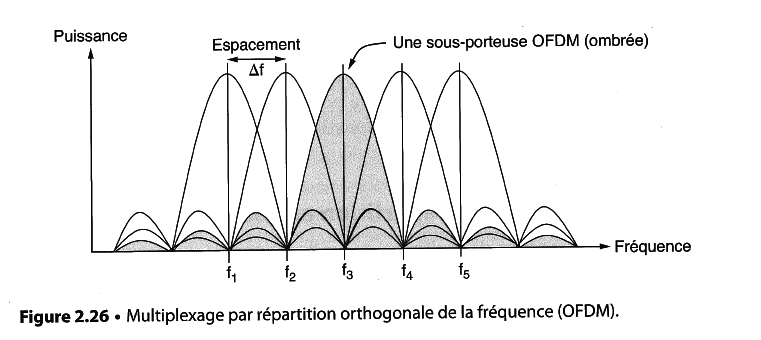
\includegraphics[width=.8\linewidth]{img/2-26.png}\\
	{\scriptsize OFDM - Image de [Tanenbaum]}
\end{center}
\end{frame}


\section{Multiplexage temporel (TDM)}

\begin{frame}[fragile]
  \frametitle{Multiplexage temporel (TDM)}
{\bf\large Multipdexage temporel \\
(\textit{TDM Time Division Multiplexing})}\\
Émission tour à tour
\begin{itemize}
	\item Chaque utilisateur émet à son tour sur l'intégralité de la bande passante
\end{itemize}
\vspace{1cm}
Exemple
\begin{itemize}
	\item Réseaux téléphoniques et cellulaires
\end{itemize}
\end{frame}

\section{Multiplexage temporel TDM}

\begin{frame}[fragile]
  \frametitle{Multiplexage temporel TDM}
\begin{center}
	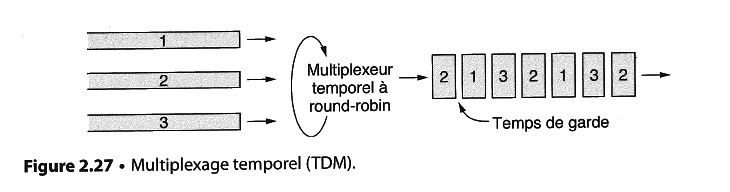
\includegraphics[width=.8\linewidth]{img/2-27.png}\\
	{\scriptsize TDM - Image [Tanenbaum]}
\end{center}
\end{frame}



\section{Multiplexage par répartition en codes CDMA}

\begin{frame}[fragile]
  \frametitle{Multiplexage par répartition en codes (CDMA)}
{\large\bf Multiplexage par répartition de codes \\
(\textit{CDMA Code Division Multiple Access})}\\
Plusieurs utilisateurs utilisent la même bande de fréquence
\begin{itemize}
	\item Tout le monde émet sur la même fréquence
	\item Plusieurs émissions se distinguent car elles sont codées différement
\end{itemize}
\end{frame}

\begin{frame}[fragile]
  \frametitle{Multiplexage par répartition en codes (CDMA)}
\textbf{Fonctionnement}
\begin{itemize}
	\item Chaque temps bit est divisé en \textit{m} courts intervalles
	(\textbf{chips})
	\item \textit{m} vaut généralement 64 ou 128 (dans l'exemple, $m=8$)
	\item Chaque station reçoit une \textbf{séquence de chips} unique et telle
	que deux séquences $S$ et $T$ quelconque ont un produit nul $S\bullet T$
	$$S\bullet T = \frac{1}{m}\sum^m_{i=1}S_iT_i$$
	\begin{itemize}
		\item Exemple (-1, -1, -1, +1, +1,-1, +1, +1)
	\end{itemize}
	\item Pour émettre 1, émission de la séquence de chips
	\item Pour émettre 0, émission de la \textbf{négation} de la séquence
\end{itemize}
\end{frame}

\begin{frame}[fragile]
  \frametitle{Multiplexage par répartition en codes (CDMA)}
\begin{center}
	\item 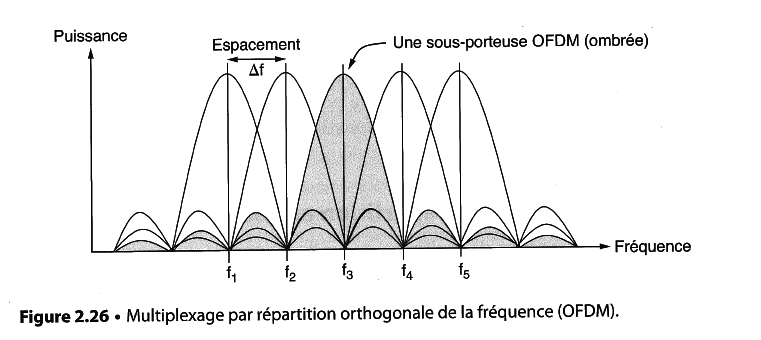
\includegraphics[width=.7\linewidth]{img/2-26.png}\\
	{\scriptsize Exemple CDMA - Image [Tanenbaum]}
\end{center}
\end{frame}

\section{Multiplexage en longueur d'ondes (WDM)}

\begin{frame}[fragile]
  \frametitle{Multiplexage en longueur d'ondes (WDM)}
{\large\bf Multiplexage en longueur d'ondes  \\
(\textit{WDM Wavelength Division Multiplexing})}
\begin{itemize}
	\item Sorte de multiplexage fréquentiel à très hautes fréquences
	\item Destiné à la fibre optique (grande bande passante)
\end{itemize}
\vspace{.5cm}
\textbf{Fonctionnement}
\begin{itemize}
	\item Chaque fibre arrive sur un prisme
	\item Les flux, d'énergie et de longueur d'onde spécifique, sont combinés
	\item À la sortie, le faisceau est séparé
\end{itemize}
\end{frame}

\begin{frame}[fragile]
  \frametitle{Multiplexage en longueur d'ondes (WDM)}
\begin{center}
	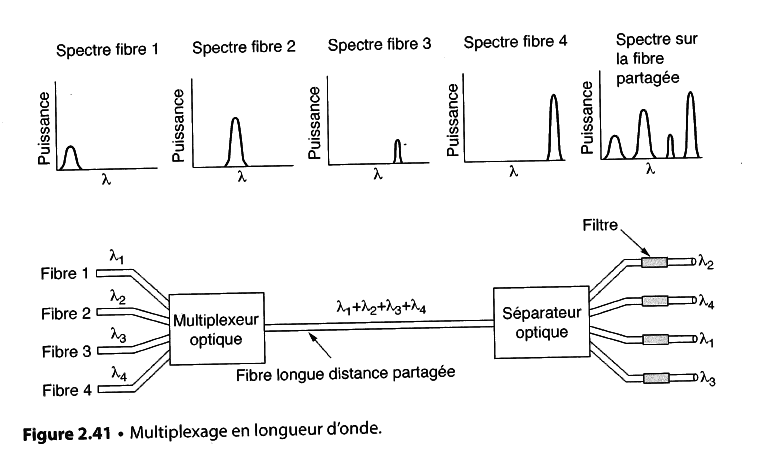
\includegraphics[width=.8\linewidth]{img/2-41.png}\\
	{\scriptsize WDM - Image [Tanenbaum]}
\end{center}
\end{frame}


